\chapter{Manual installation}
\label{chapter:manual_install}

\section{Introduction}
The manual installation can be done on both Microsoft Windows 2000 or higher or a Linux distribution with the following software pre-installed : 
\begin{itemize}
\item Sun Java2 Standard Edition version 5.0 or higher
\item Apache Tomcat Core 5.5 or higher (other Servlet containers might work, but are not officially supported yet)
\item Postgresql 8.2.4 or higher
\end{itemize}
If you have no experience installing this software, please consult your local system administor.

\section{Manual installation steps}
\subsection{Configuring the Postgresql database}
Log in as posgres administrator to psql
\\
\\
Create a new role:
\\
\textbf{create user \textit{role\_name} password '\textit{role\_password}';}
\\
\\
Create a new database:
\\
\textbf{create database regadb owner \textit{role\_name};}
\\
\\
Create the schema:
\\
\textbf{create schema regadbschema authorization \textit{role\_name};}
\\
\\
Log out from psql
\\
\\
Create the Postgres database structure (this file can be downloaded from the RegaDB website)
\\
\textbf{psql -U \textit{role\_name} regadb -f posgresSchema.sql}

\subsection{RegaDB configuration}
Download the global-conf.xml file from the RegaDB website. This config file can be placed at the default location (/etc/rega\_institute/regadb), or at an alternative location.

If you place the configuration file at an alternative location, you should define an environment variable called \textbf{REGADB\_CONF\_DIR} containing this path.
Following attributes of the XML file should be filled in:
\begin{itemize}
\item hibernate.connection.driver\_class : the default value is correct, do not change this
\item hibernate.connection.password : replace default by your \textit{role\_password}
\item hibernate.connection.url : replace default by the URL of your Postgresql database + /regadb (eg. jdbc:postgresql://serverName:5432/regadb)
\item hibernate.connection.username : replace default by your \textit{role\_name}
\item hibernate.dialect : the default value is correct, do not change this
\item regadb.query.resultDir : replace default by a directory where query results should be stored (eg. /soft/regadb/queryResults), this directory should be writable by your servlet container
\item http.proxy.url : replace default by your proxy server name, if you have direct access to internet, simply remove default
\item http.proxy.port : replace default by your proxy server port, if you have direct access to internet, simply remove default
\end{itemize}

Note that this file should only be accessible by your servlet container, so please make sure only your servlet container user has read access to it.

\lstset{language=XML, caption={RegaDB XML configuration file example (with proxy settings)}}
\begin{lstlisting}
<?xml version="1.0" encoding="UTF-8"?>
<regadb-settings>
  <property name="hibernate.connection.driver_class">
		org.postgresql.Driver
	</property>
  <property name="hibernate.connection.password">
		nock_nock
	</property>
  <property name="hibernate.connection.url">
		jdbc:postgresql://zolder:5432/test_regadb
	</property>
  <property name="hibernate.connection.username">
		woody
	</property>
  <property name="hibernate.dialect">
		org.hibernate.dialect.PostgreSQLDialect
	</property>
  <property name="regadb.query.resultDir">
		/soft/regadb/queryResults
	</property>
  <proxy>
    <property name="http.proxy.url">
			www-proxy
		</property>
    <property name="http.proxy.port">
			3128
		</property>
  </proxy>
</regadb-settings>
\end{lstlisting}

\lstset{language=XML, caption={RegaDB XML configuration file example (no proxy settings)}}
\begin{lstlisting}
<?xml version="1.0" encoding="UTF-8"?>
<regadb-settings>
  <property name="hibernate.connection.driver_class">
    org.postgresql.Driver
  </property>
  <property name="hibernate.connection.password">
    nock_nock
  </property>
  <property name="hibernate.connection.url">
    jdbc:postgresql://zolder:5432/test_regadb
  </property>
  <property name="hibernate.connection.username">
    woody
  </property>
  <property name="hibernate.dialect">
    org.hibernate.dialect.PostgreSQLDialect
  </property>
  <property name="regadb.query.resultDir">
    /soft/regadb/queryResults
  </property>
  <proxy>
    <property name="http.proxy.url">
    </property>
    <property name="http.proxy.port">
    </property>
  </proxy>
</regadb-settings>
\end{lstlisting}

\subsection{Deploy RegaDB into your servlet container}
Download the regadb.war file from the RegaDB website.
\\
Navigate your browser to the Tomcat welcome page (f.e. http://serverName:8080/).
\\
\vspace{0.5cm}~ \\ \centerline{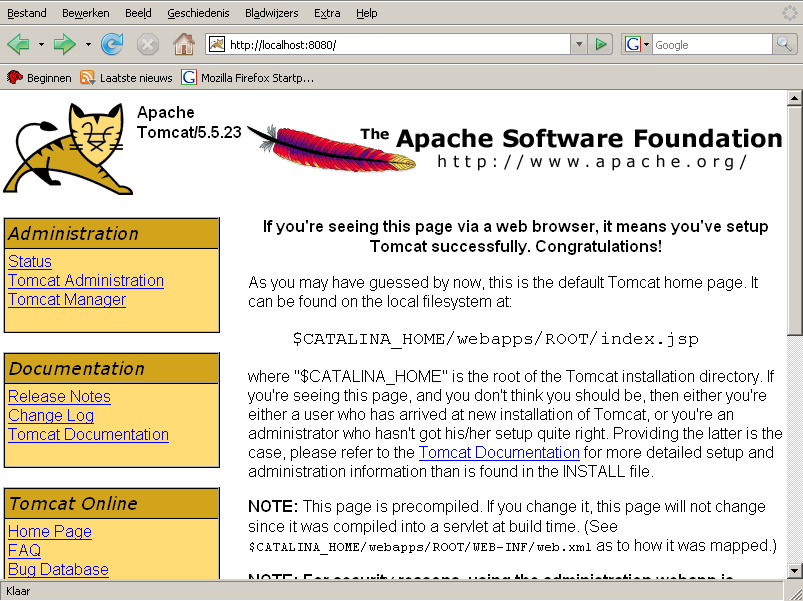
\includegraphics[width=8cm] {pics/nsis/tomcat_page.png}}
Navigate to the manager page and fill in the proper username and password.
\\
\vspace{0.5cm}~ \\ \centerline{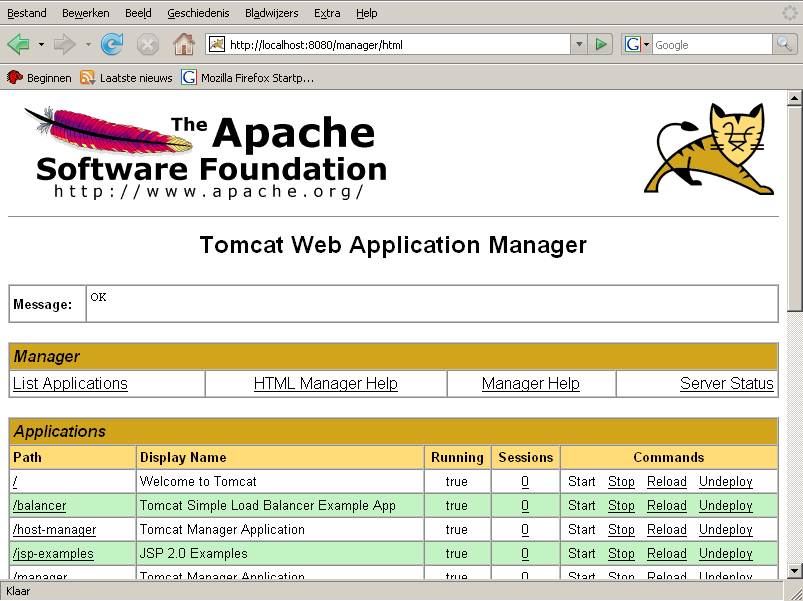
\includegraphics[width=8cm] {pics/nsis/tomcat_page_manager_1.png}}
Go to the Deploy section, browse for the regadb.war file and click \textbf{Deploy}. RegaDB will be deployed in the servlet container, this might take a few minutes.
\\
\vspace{0.5cm}~ \\ \centerline{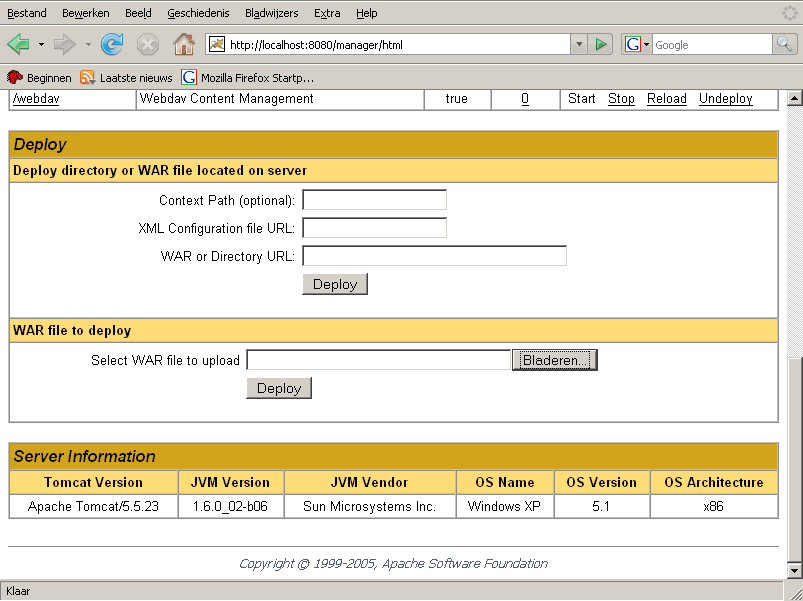
\includegraphics[width=8cm] {pics/nsis/tomcat_page_manager_2.png}}

\subsection{Initiating the database}
Download the regadb-install.tgz archive, and extract this archive to a temporary directory. 
Navigate to this directory and execute regadb-install-regadb-init.jar;
\\\textbf{java -jar regadb-install-regadb-init.jar}

This command will initialize the RegaDB database. Please proceed to the Post installation chapter to finish the RegaDB configuration (chapter~\ref{chapter:post_install}).
